% !TeX root = Logpp.tex
Given the design principals outlined in \autoref{sec:implementation} we now 
present the implementation of \projn\footnote{\projn sources available at 
\url{https://github.com/mrkmarron/logpp}} which realizes these goals in a logger 
for the \texttt{Node.js}~\cite{Node} runtime. It is possible to implement many 
of the features needed to satisfy our design goals as a library or using the 
native API extension bindings (N-API~\cite{NAPI}) but others require core 
runtime support. For these core changes we modify the ChakraCore JavaScript 
engine and core Node implementation directly.

\subsection{Implementation Overview}
The logging system is split into five major components that (1) manage the 
global logger states, message formats, and activities (2) the in-memory logger 
(3) the stage processor (4) the formatter (5) and finally the emitter. These 
components and the relations between them are shown in~\autoref{fig:arch} and 
explained in detail in the rest of the section. We will also use a running 
example in~\autoref{fig:runningExample} to illustrate various aspects of the 
system.

\begin{figure}
    \centering
    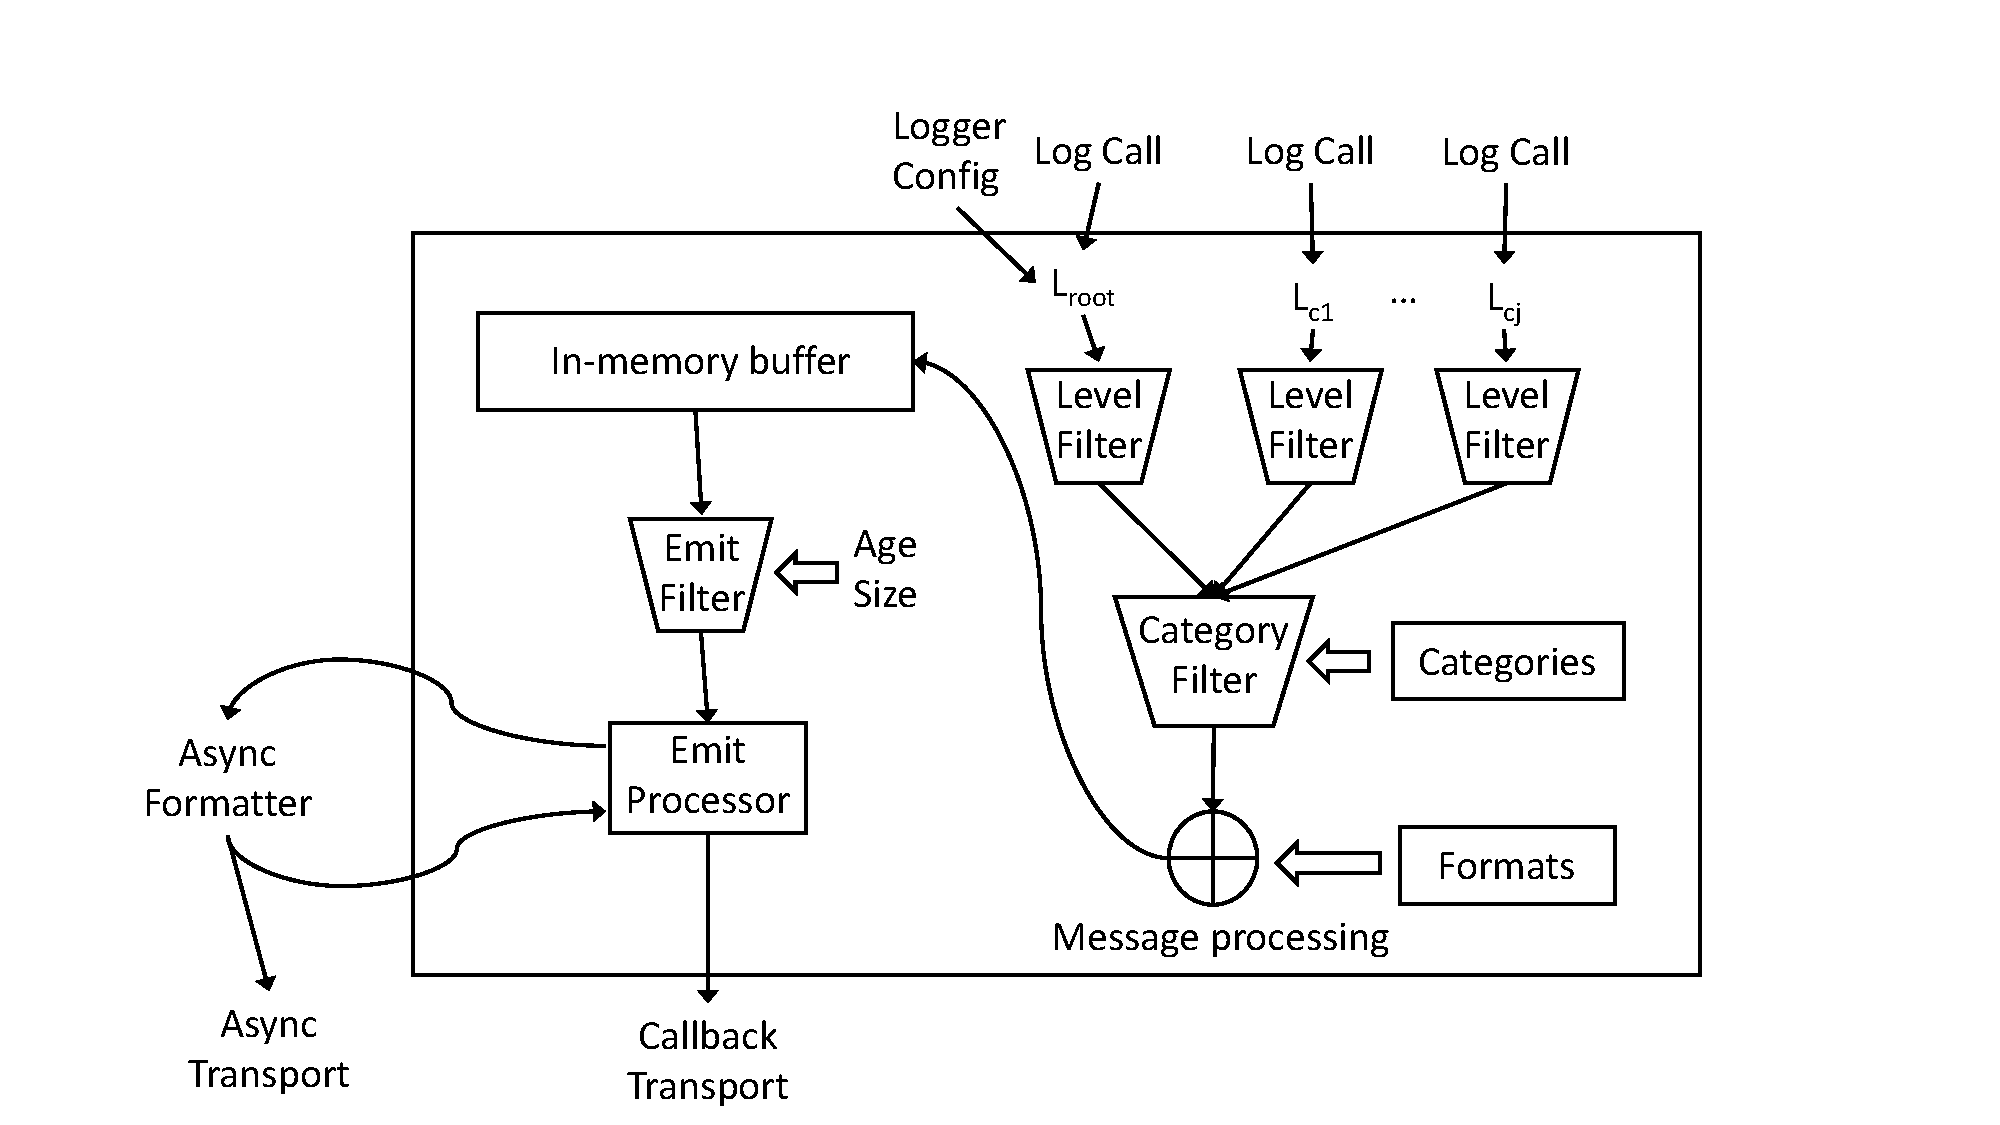
\includegraphics[width=0.5\textwidth,angle=-90]{Figures/ArchDiagram}
    \caption{Logger architecture}
    \label{fig:arch}
\end{figure}

\begin{figure*}[t]
\begin{minipage}[b]{0.47\textwidth}
    \lstinputlisting[language=JavaScript,basicstyle=\scriptsize]{Code/runningExample.js} 
    \caption{Main app code}
    \label{fig:appmain}
\end{minipage}
\begin{minipage}[b]{0.47\textwidth}
    \lstinputlisting[language=JavaScript,basicstyle=\scriptsize]{Code/runningExampleSub.js}
    \caption{Submodule code}
    \label{fig:appsub}
\end{minipage}
\caption{Running example}
\label{fig:runningExample}
\end{figure*}

\subsection{JavaScript Implementation}
\paragraph{Log State Manager}
\noindent
The first component we look at in the implementation is the global log state 
manager. This component is responsible for tracking all of the loggers that 
have been created, which is the root logger, the enabled logging levels + 
categories, and the message formats which have been defined. 

As seen in~\autoref{fig:arch} and the running example may be many loggers 
created in different parts of the application. One logger is created on line 
2 of the main application~\autoref{fig:appmain} while a second is created 
in the module \texttt{foo.js} in~\autoref{fig:appsub} which is included from 
the main \texttt{app.js} file. As stated in \emph{design principle 5} we 
do not want the included sub-module \texttt{foo.js} to be able to, unexpectedly, 
change the logging level for the main app (the call to \texttt{setOutputLevel} on 
line 9). We also want to allows the root logger to enable/disable log outputs 
from these subloggers.

To support these features the \projn logger keeps a list of all created loggers 
and a special \emph{root logger} which is the first logger created in the main 
module of the application. When updating logging levels or creating a new logger 
we check if action is comming from the root logger and, if not, either convert 
the call to a \texttt{nop} or look at the root logger configuration to see if 
we need to override any parameters.

In our running example the state manager will intercept the creation of the logger 
on line 2 in \texttt{foo.js}. Since the logger created here is not the root logger
the state manager will intercept this construction, set the in-memory log level to 
the overridden \texttt{WARN} level instead of the default value of \texttt{DETAIL}, 
prevent the modification of the \emph{emit-level} or the output sink, and will 
store the newly created logger in a list of sub-loggers. 

Tracking the list of all created sub-loggers also allows a developer to share a 
single logger between several files in the same module. The name parameter in the 
logger constructor is keyed with the logger and, if the same key is used in multiple 
places, the same logger object will be returned.

Finally, the state manager is responsible for maintaining information on the current 
\emph{emit level}, the enabled/disabled categories, and the sublogger override information. 
Each logger has an independent level at which it can write into the in-memory log but 
the state manager maintains a global set of enabled/disabled categories which each logger 
uses and a global logging level for eventual emit processing. Only the root logger is 
allowed to update the categories and emit levels. 

In our running example the main application has a log statement on lines $12$ and $14$ 
that are in the \texttt{Perf} category and will put a message with the current walltime 
in the log. As the first log statement happens before the \texttt{Perf} category has 
been enabled it will not be processed. However, after enabling the \texttt{Perf} category 
on line $13$ the log operation on line $14$ will be processed and result in a message 
being saved to the in-memory log.

\paragraph{Message Formats}
\noindent
To improve performance and enable the log output to be easily machine parsed we 
adopt a \emph{semantic logging} approach where the log call copies the format 
information and message arguments to a secondary location instead of formatting them 
immediately. Since the copy operation is very low cost this minimizes the 
performance impact on the main thread and allows the formatter to build up a 
parser for all the messages it emits which can be later used to parse the log. 
Modern software development also favors the use of consistent styles and data 
values in the log. Thus, \projn encourages developers to split the logging 
action into two components:
\begin{itemize}
\item Format definition using the \texttt{addFormat} method which takes a format 
string or JSON format object, processes it into an optimized representation, 
and then saves it for later use.
\item Format use in a log statment which takes a format identifier and a list of 
arguments, and then, processes them.
\end{itemize}

In addition to programtically processing single log formats, as shown on line 3 
in~\autoref{fig:appmain}, we also allow the programmer to load formats in bulk 
from a JSON formatted file. This allows a team to have a unified set of logging 
messages that can be loaded/processed quickly on startup and then used repeatedly 
throughout the applications execution. Once loaded all format objects are saved 
in the \emph{formats} component in~\autoref{fig:arch} where they can be loaded 
as needed for processing a log statement.

The format for a logger message is:
\begin{lstlisting}[language=JavaScript,basicstyle=\scriptsize]
{
  formatName: string, //name of the format
  formatString: string, //raw format string
  formatterEntries: {
    kind: number, //tag indicating the entry kind
    argPosition?: number, //position in argument list
    expandDepth?: number, //JSON expand depth
    expandLength?: number //JSON expand length
  }[]
}
\end{lstlisting}

This representation allows us to quickly scan an process the arguments as 
described in the \emph{Message In-Memory Processing} section. The kind 
information is used for both identifying what type of value is expected 
when formatting an argument, e.g. \texttt{number}, \texttt{string}, etc., 
but we also use it to support \emph{format macros}.

To support the easy/efficient logging on a number of common values that 
are not easily (or cheaply) computable we provide \emph{format macros}. 
Classic examples include adding the current walltime or the hostname as 
part of a log message. In JavaScript these require explicitly calling 
expensive compund API sequences \texttt{new Date().toISOString()} or 
\texttt{require('os').hostname()}. Instead we allow a developer to use 
special macros \texttt{\#walltime}, as seen on line 11 in~\autoref{fig:appmain}, 
or \texttt{\#host} in their format 
strings and then the logger has optimized internal paths to get the needed 
values. In these cases the \texttt{kind} field is set to the enumeration 
for the macro and the \texttt{argPosition} is undefined.

A common logging practice is to include raw objects, formatted as JSON, into the 
message. This is a convinient way to include rich data into a message but can 
lead to unexpectedly large logging loads when, what the developer expected to 
be a small object, turns out to be quite large. To prevent this we have a specialized 
JSON-style processor that will bound the depth/length of object expansion during 
formatting. The \texttt{expandDepth} and \texttt{expandLength} arguments provide 
control over this depth/length and can be adjusted in the format string when a 
developer want to capture more (or less) information than what is provided by the 
defaults.

\paragraph{Message In-Memory Processing}
\noindent
The in-memory buffer is implemented as a linked-list of block structures:
\begin{lstlisting}[language=JavaScript,basicstyle=\scriptsize]
{
  tags: Uint8Array,
  data: Float64Array,
  strings: string[],
  properties: map<number, string>
}
\end{lstlisting}

To allow efficient marshalling of the data from our JavaScript logger frontend 
to the C++ N-API code that handles the formatting we encode all values into 
$64$bit based representation (stored in the \texttt{data} property). We use a set 
of enumeration \texttt{tags} (stored in the \texttt{tags} property) to track 
what kind of value the corresponding $64$bit value represents. We have special 
handling for string and object properyt values, described below, that use the 
\texttt{strings} array and \texttt{properties} map to index and keep alive these values.

When implementing a sematic logging system the key invariant that needs to be 
preserved is that the values of each argument must not be changed between the 
time when the log call happens and when the argument is processed for 
formatting. Certain values including booleans, numbers, and strings, are 
immutable according to the language semantics so we can just copy the 
references directly into our in-memory array. However, in cases where the 
argument is a mutable object we must take explicit actions. A simple solution 
would be to JSON \texttt{stringify} the argument immedaitely, and while this 
prevents mutation and allows semantic formatting, it comprimises possible 
performance gains we are looking for. Instead we recursively flatten the object 
into the in-memory buffer with the code shown here:
\lstinputlisting[language=JavaScript,basicstyle=\scriptsize]{Code/flatten.js}

This code represents the transition from the \emph{formats} and \emph{arguments} 
inputs into the \emph{in-memory buffer} shown in~\autoref{fig:arch}. This code 
starts off by checking if we are either in a cycle or the depth bound has been 
reached. If either of these occour we put a special tag, \texttt{CycleTag} or 
\texttt{DepthBoundTag} respectively, into the tags array and return. If not we 
continue with the pre-order traveral of the object graph by updating the cycle 
info, adding the special \texttt{LParenTag} to the buffer, and enumerating the 
object properties. For each property we check if the length bound is met, adding 
the special \texttt{LengthBoundTag} and breaking if needed, if not we add the 
property and value information to the in-memory buffer. The property value \texttt{p} 
is a special string value which is very likely to be repeated so we use a map 
from properties to unique numeric identifiers to compress and convert them into 
a number which can be stored in the \texttt{data} component of the in-memory buffer 
via the \texttt{addPropertyEntry} function. The value associated is recursively 
processed via the \texttt{addGeneralEntry} call which switches on the type of the 
value, booleans and numbers are converted directly to \texttt{Float64} representations, 
strings are mapped by index in the \texttt{strings} array, and \texttt{Date} objects 
are converted to $64$bit timestamps using the \texttt{valueOf} method. Similar to 
standard JSON formatting other values are simplified but, instead of just dropping 
them, we use a special \texttt{OpaqueValueTag}. After all the properties have 
been processed we update the cycle tracking information and add a closing 
\texttt{RParenTag}.

\begin{figure}
    \centering
    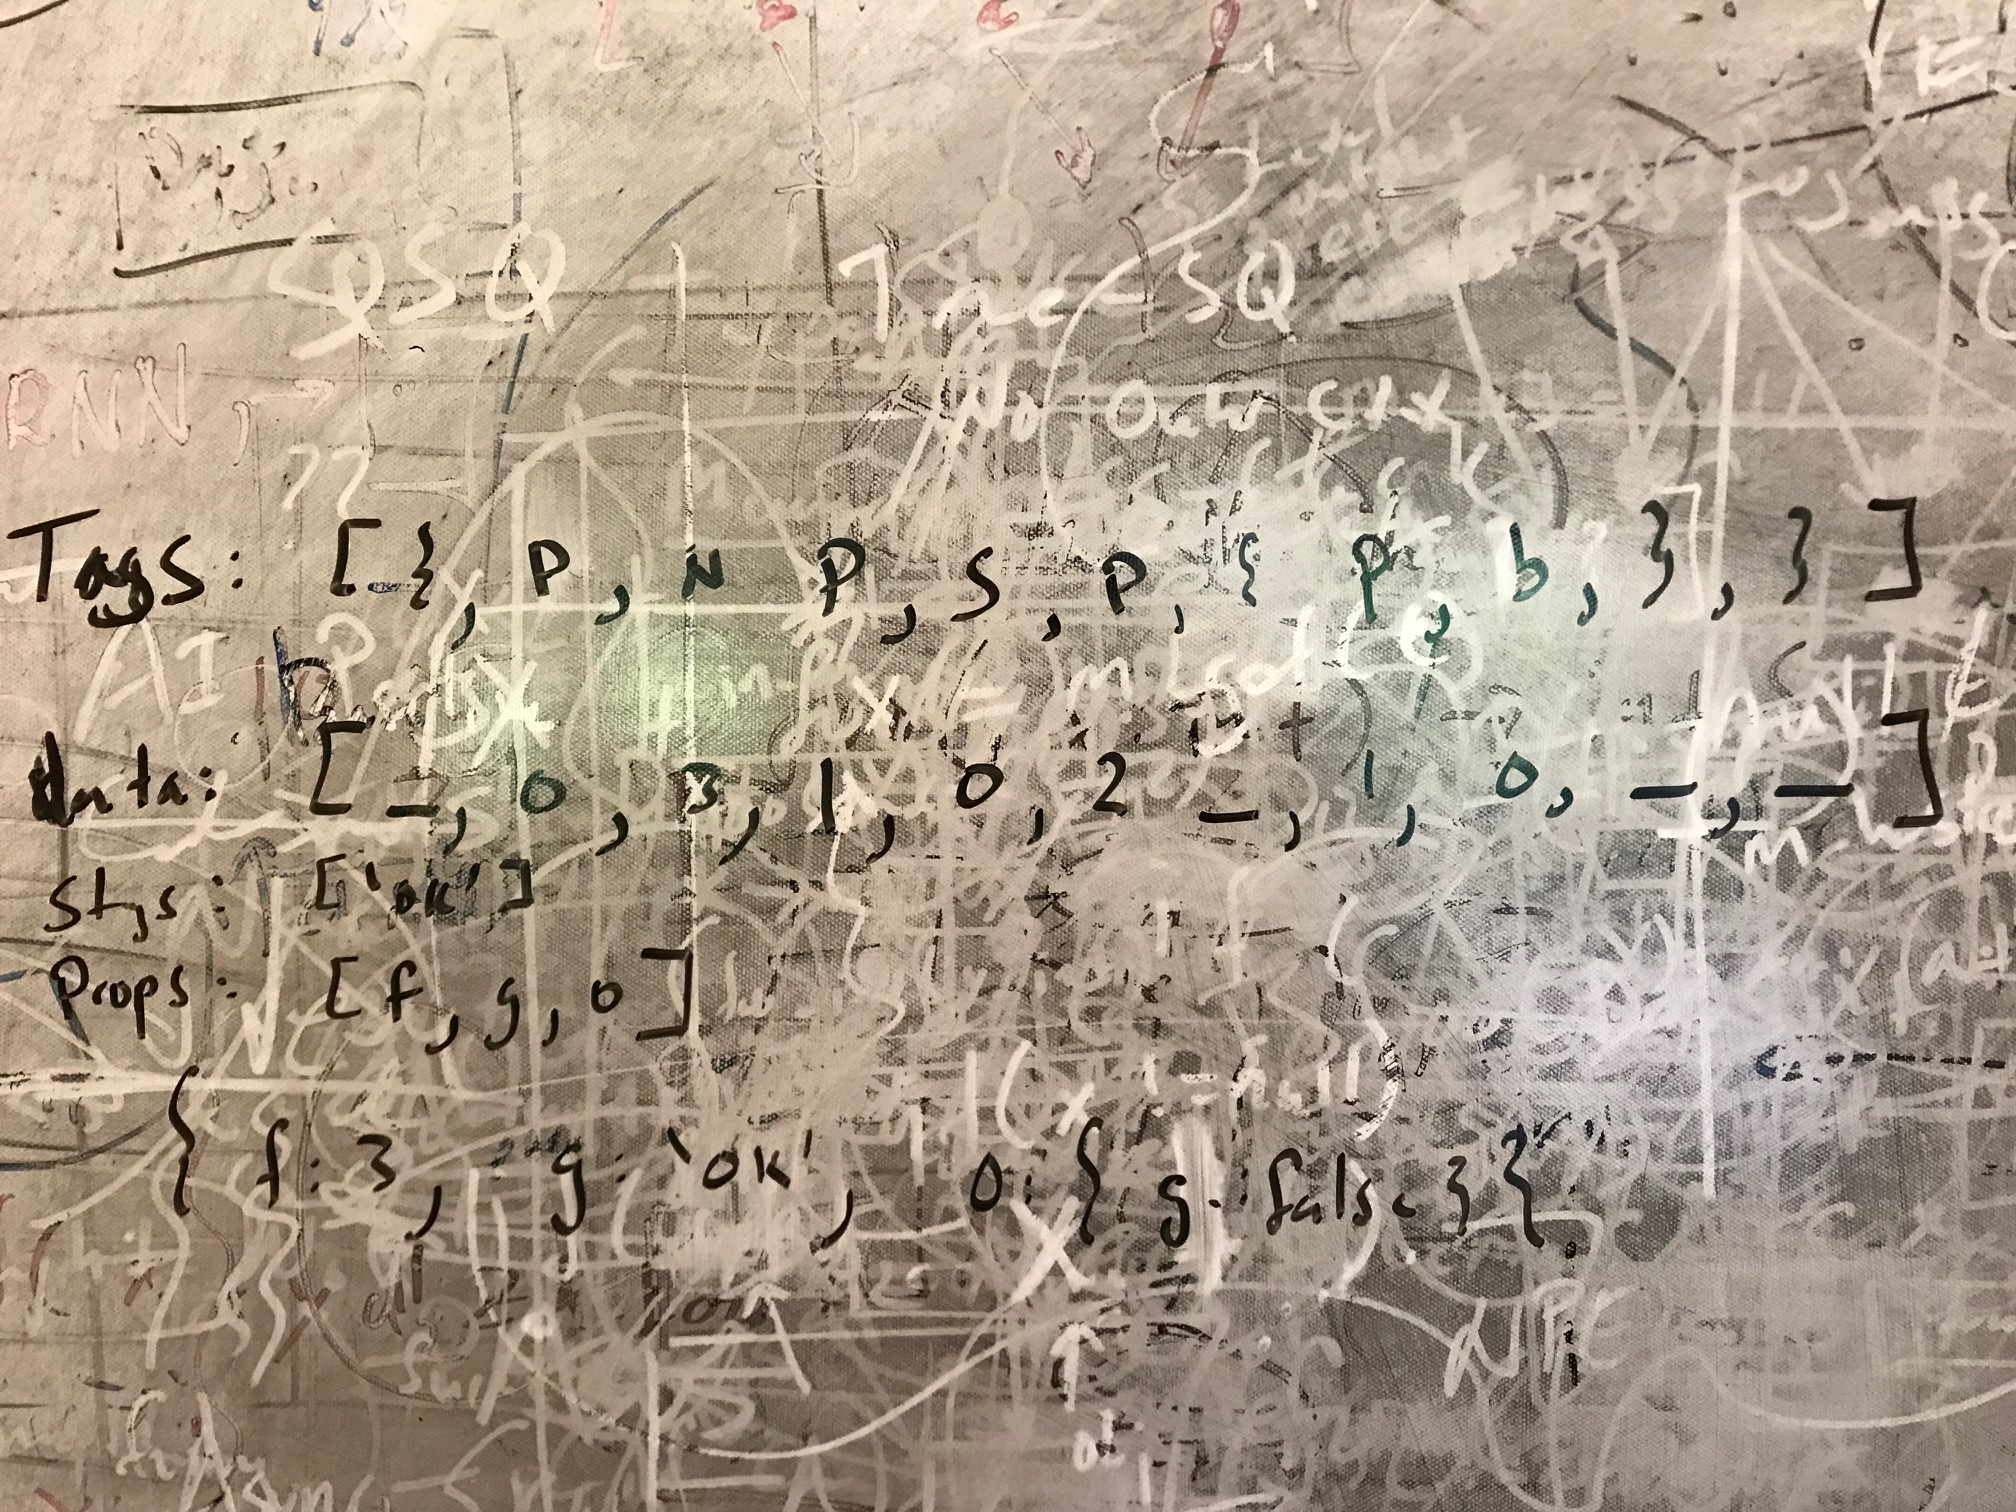
\includegraphics[width=0.5\textwidth]{Figures/InMemoryExample}
    \caption{In-Memory buffer processing example}
    \label{fig:inmemory}
\end{figure}

To illustrate how this code works in practice consider the case of processing the 
object argument:

\begin{lstlisting}[language=JavaScript,basicstyle=\scriptsize,numbers=none]
{
  f: 3,
  g: 'ok',
  o: { g: false, id: (x) => x }
}
\end{lstlisting}

The resulting state of the in-memory buffer is shown in~\autoref{fig:inmemory}. 
In this example we can see how the object structure has been flattened into 
the buffer with the \lstinline!'{'! and \lstinline!'}'! tags denoting the bounds 
of each object. Each of the properties has been registered in the map (with a fresh 
numeric identifier) and this is stored in the \texttt{data} array. For example the 
property \lstinline!g! is mapped to $1$ and in both occournces in the object 
structure the entry in the \texttt{tags} array is set to \lstinline!'p'! for 
property and the value in the \texttt{data} array is set to match the corresponding 
numeric identifier $1$. The numeric and boolean values are mapped in the obvious 
way, directly for the number and to $0$/$1$ for the boolean with the appropriate 
tag values set. Similar to the properties the string value \lstinline!'ok'! is 
mapped to an integer index, index $0$, in the \texttt{strings} array. Finally, 
since functions are not serializable, the value associated with the \lstinline!id! 
property is dropped and we simply store the \texttt{OpaqueValueTag} (\lstinline!'?'!) 
in the corresponding position of the \texttt{tags} array.

\paragraph{Message Staging and Emit}
\noindent

make sure to discuss callbacks + on demand synchrous emit

also detailed emit on "unusual" events

\paragraph{Logging APIs}
\noindent

\subsection{Native C++ Implementation}

Background N-API formatter

Background uploads

\subsection{Custom Runtime Implementation}

Format checking

Mutability checking

Code regen on level changes

Fast string + property handling

